% Options for packages loaded elsewhere
\PassOptionsToPackage{unicode}{hyperref}
\PassOptionsToPackage{hyphens}{url}
%
\documentclass[
]{article}
\usepackage{lmodern}
\usepackage{amssymb,amsmath}
\usepackage{ifxetex,ifluatex}
\ifnum 0\ifxetex 1\fi\ifluatex 1\fi=0 % if pdftex
  \usepackage[T1]{fontenc}
  \usepackage[utf8]{inputenc}
  \usepackage{textcomp} % provide euro and other symbols
\else % if luatex or xetex
  \usepackage{unicode-math}
  \defaultfontfeatures{Scale=MatchLowercase}
  \defaultfontfeatures[\rmfamily]{Ligatures=TeX,Scale=1}
\fi
% Use upquote if available, for straight quotes in verbatim environments
\IfFileExists{upquote.sty}{\usepackage{upquote}}{}
\IfFileExists{microtype.sty}{% use microtype if available
  \usepackage[]{microtype}
  \UseMicrotypeSet[protrusion]{basicmath} % disable protrusion for tt fonts
}{}
\makeatletter
\@ifundefined{KOMAClassName}{% if non-KOMA class
  \IfFileExists{parskip.sty}{%
    \usepackage{parskip}
  }{% else
    \setlength{\parindent}{0pt}
    \setlength{\parskip}{6pt plus 2pt minus 1pt}}
}{% if KOMA class
  \KOMAoptions{parskip=half}}
\makeatother
\usepackage{xcolor}
\IfFileExists{xurl.sty}{\usepackage{xurl}}{} % add URL line breaks if available
\IfFileExists{bookmark.sty}{\usepackage{bookmark}}{\usepackage{hyperref}}
\hypersetup{
  hidelinks,
  pdfcreator={LaTeX via pandoc}}
\urlstyle{same} % disable monospaced font for URLs
\usepackage[margin=1in]{geometry}
\usepackage{graphicx}
\makeatletter
\def\maxwidth{\ifdim\Gin@nat@width>\linewidth\linewidth\else\Gin@nat@width\fi}
\def\maxheight{\ifdim\Gin@nat@height>\textheight\textheight\else\Gin@nat@height\fi}
\makeatother
% Scale images if necessary, so that they will not overflow the page
% margins by default, and it is still possible to overwrite the defaults
% using explicit options in \includegraphics[width, height, ...]{}
\setkeys{Gin}{width=\maxwidth,height=\maxheight,keepaspectratio}
% Set default figure placement to htbp
\makeatletter
\def\fps@figure{htbp}
\makeatother
\setlength{\emergencystretch}{3em} % prevent overfull lines
\providecommand{\tightlist}{%
  \setlength{\itemsep}{0pt}\setlength{\parskip}{0pt}}
\setcounter{secnumdepth}{-\maxdimen} % remove section numbering
\usepackage{hyperref} \usepackage{booktabs} \hypersetup{ colorlinks=true, linkcolor=blue, filecolor=magenta, urlcolor=cyan}
\newlength{\cslhangindent}
\setlength{\cslhangindent}{1.5em}
\newenvironment{cslreferences}%
  {\setlength{\parindent}{0pt}%
  \everypar{\setlength{\hangindent}{\cslhangindent}}\ignorespaces}%
  {\par}

\author{}
\date{\vspace{-2.5em}}

\begin{document}

\newpage
\begin{flushright}
    \textbf{Équipe 8}
\end{flushright}

\begin{center}
    \vspace{2\baselineskip}
    Charles Comeau \\
    (111 185 421) \\
    \vspace{1\baselineskip}
    Nicholas Langevin \\
    (111 184 631) \\
    \vspace{1\baselineskip}
    Andréanne Larouche \\
    (111 190 518) \\
    \vspace{7\baselineskip}
    Apprentissage statistique en actuariat\\
    ACT-3114 \\
    \vspace{7\baselineskip}
    {\large
    \textbf{Analyse des données de renouvellement d'assurance}} \\
    \vspace{8\baselineskip}
    présenté à \\
    Marie-Pier Côté \\
    \vspace{9\baselineskip}
    École d’actuariat \\
    Université Laval \\
    27 février 2020
\end{center}

\newpage

\tableofcontents

\newpage

\hypertarget{introduction}{%
\section{Introduction}\label{introduction}}

Les données qui seront analysées dans ce rapport proviennent du jeu de
données ``eudirectlapse'' du paquetage ``CASdatasets'' de R. Dans le but
de modéliser le statut de renouvellement de polices d'assurance,
représenté par la variable ``lapse'' dans ce cas-ci, il sera d'abord
nécessaire de visualiser et de prétraiter les données observées des 23
060 polices d'assurance. Il est à noter que la durée d'observation est
de un an et que l'année visée et la compagnie demeurent inconnues. On
pourra distinguer les statuts de renouvellement comme étant affiché à
résigné (``Resignation''``) ou à renouvellement (''Renouvellement")
selon le cas approprié. Ce jeu de données est intéressant du fait qu'il
permettra au fur de l'analyse de nous indiquer les variables types ayant
un impact sur la décision de renouvellement de police des assurés d'une
compagnie d'assurance X. En plus d'être un problème de nature
actuarielle, le jeu de données choisi pourra nous permettre d'entamer
une ouverture des réflexions possibles lorsque nous aurons à travailler
dans une compagnie d'assurance. Étant trois personnes intéressées par
l'assurance de dommages, ce problème nous semblait des plus appropriés
et intéressant face à nos intérêts communs. Le nombre d'observations est
également intéressant, car il nous permettra de porter des conclusions
précises avec assez de crédibilité sans toutefois être avoir à
travailler avec un jeu de données inutilement trop volumineux. De plus,
chaque variable explicative semble à prime à bord intéressante pour
l'analyse et assez pertinente, ce que nous pourrons découvrir dans
l'élaboration de ce travail pratique.

\newpage

\hypertarget{analyse-exploratoire-des-donnuxe9es}{%
\section{Analyse exploratoire des
données}\label{analyse-exploratoire-des-donnuxe9es}}

\hypertarget{variable-ruxe9ponse}{%
\subsection{Variable réponse}\label{variable-ruxe9ponse}}

La variable \textbf{lapse} indique si l'assuré à renouveler ou non sa
police lors du renouvellement. Il s'agit de la variable exogène.
Initialement, le choix du client était indiqué par une variable binaire.
Si le client désirait résigner sa police lapse prenait la valeur 1,
autrement elle prenait la valeur 0. À des fins de simplification et pour
que la visualisation en soit améliorée pour la suite, nous avons
converti la variable en variable catégorielle à deux niveaux. La
variable prendra maintenant la valeur \textbf{resignation} si le client
résigne sa police et de \textbf{renouvellement} s'il la renouvelle.

On constate qu'il y a 23060 clients dont 20106 qui ont renouveler leur
police d'assurance, ce qui représente une proportion de 87.19\%. La
variable réponse n'est donc pas symétrique et il sera important d'en
tenir compte lors de la modélisation. L'analyse des variables
explicatives contenues dans ce jeu de données nous permettra de mieux
comprendre les causes de résignation et de créer des patrons pour ainsi
arriver à bien modéliser la variable de renouvellement de police.

\hypertarget{variables-catuxe9gorielles-nominales}{%
\subsection{Variables catégorielles
nominales}\label{variables-catuxe9gorielles-nominales}}

La variable \textbf{polholder\_diffdriver} représente la différence de
statut qui pourrait avoir entre le propriétaire de la police et le
conducteur principal.

\begin{table}[ht]
\centering
\caption{Distribution de la différence de statut entre le conducteur et le détenteur de la police} 
\label{tbl:statutdiff}
\begin{tabular}{lcr}
  \hline
Statut & Nombre d'observation & Distribution \\ 
  \hline
Conducteurs agée de 24+ & 1728 & 7.49 \% \\ 
  Commerciale & 40 & 0.17 \% \\ 
  Conducteur apprenti de 17 ans & 42 & 0.18 \% \\ 
  Partenaire de couple & 8128 & 35.25 \% \\ 
  Utilisateur seul & 11155 & 48.37 \% \\ 
  Jeunes utilisateurs & 1955 & 8.48 \% \\ 
  Données manquantes & 12 & 0.05 \% \\ 
   \hline
\end{tabular}
\end{table}

\textless\textless\textless\textless\textless\textless\textless{}
HEAD:01-Rapport.Rmd On constate que la plupart des voitures assurées est
utilisée seulement par le détenteur de la police ou par l'assuré et son
partenaire de couple puisque c'est deux cas représente 83.62\% des
observations. Il y a un pourcentage non négligeable de 8.48\% pour
lequel le véhicule est partagé par de jeunes conducteurs alors qu'il y a
7.49\% des cas ou le véhicule est plutôt partagé entre des personnes
plus agées (24 ans et plus). À noter qu'il y a 12 observations pour
lesquelles la variable est manquante. Cela sera traité dans la section
traitement des valeurs manquantes. ======= On constate que la plupart
des voitures assurées est utilisée seulement par le détenteur de la
police ou par l'assuré et son partenaire de couple puisque c'est deux
cas représente 83.62\% des observations. Il y a un pourcentage non
négligeable de 8.48\% pour lequel le véhicule est partagé par de jeunes
conducteurs alors qu'il y a 7.49\% des cas ou le véhicule est plutôt
partagé entre des personnes plus agées (24 ans et plus). À noté qu'il y
a 12 observations pour lesquelles la variable est manquante. Cela sera
traité dans la section traitement des valeurs manquantes.
\textgreater\textgreater\textgreater\textgreater\textgreater\textgreater\textgreater{}
60809fcbf121cda8bf1ec803d70809dfdf626020:rapport1/01-Rapport.Rmd

La variable \textbf{polholder\_gender} représente le sexe du
propriétaire de la police. Voici la répartition en pourcentage du sexe
pour les propriétaires de police d'assurance.

\begin{table}[ht]
\centering
\caption{Distribution du sexe du détenteur de police} 
\label{tbl:polholderGender}
\begin{tabular}{lcr}
  \hline
Sexe & Nombre d'observation & Distribution \\ 
  \hline
Homme & 14721 & 63.84 \% \\ 
  Femme & 8339 & 36.16 \% \\ 
   \hline
\end{tabular}
\end{table}

On voit qu'il y a significativement plus d'hommes ayant une police
d'assurance chez cet assureur que de femme.

La variable \textbf{polholder\_job} est, quant à elle, celle décrivant
le travail du propriétaire du contrat. Deux valeurs sont possibles soit
``medical'' soit ``normal''. On constate que 41.12\% des assurés on un
travail de type médical alors qu'il y en a 58.88\% qui ont un autre type
d'emploi.

La variable \textbf{policy\_caruse} représente les fins d'utilisation du
véhicule.

\begin{table}[ht]
\centering
\caption{Distribution de l'utilisation du véhicule} 
\label{tbl:policyCaruse}
\begin{tabular}{lcr}
  \hline
Usage & Nombre d'observation & Distribution \\ 
  \hline
Commerciale & 10 & 0.04 \% \\ 
  Privé ou aller travailler & 19567 & 84.85 \% \\ 
  Données manquantes & 3483 & 15.10 \% \\ 
   \hline
\end{tabular}
\end{table}

On constate qu'il y a un nombre considérable de données manquantes et
très peu de véhicules pour un usage commercial.

De sont côté, la variable \textbf{vehicl\_garage} décrit le type de
stationnement de la voiture. Voici la répartition des types de
stationnements.

\begin{table}[ht]
\centering
\caption{Distribution du type de stationnement} 
\label{tbl:policyGarage}
\begin{tabular}{lcr}
  \hline
Moyen de stationnement & Nombre d'observation & Distribution \\ 
  \hline
Sous un abri d'auto & 1413 & 6.13 \% \\ 
  Terrase de stationnement & 2243 & 9.73 \% \\ 
  Stationnement privé & 199 & 0.86 \% \\ 
  Garage & 8863 & 38.43 \% \\ 
  Rue & 5468 & 23.71 \% \\ 
  Garage sous-terrain & 1056 & 4.58 \% \\ 
  Autre & 2243 & 9.73 \% \\ 
  Données manquantes & 1575 & 6.83 \% \\ 
   \hline
\end{tabular}
\end{table}

On voit que pour les moyens de stationnement les plus populaires sont le
garage privé et la rue. Il y a des données manquantes, elles seront
traitées plus loin dans le rapport.

La variable \textbf{polholder\_BMCevol} indique si la prime de
renouvellement a connu une hausse, une baisse ou est demeurée stable par
rapport à la prime payée lors du dernier renouvellement.

\begin{table}[ht]
\centering
\caption{Distribution de l'indice Bonus-Malus} 
\label{tbl:policyBM}
\begin{tabular}{lcr}
  \hline
Prime de renouvellement & Nombre d'observation & Distribution \\ 
  \hline
Hausse & 869 & 3.77 \% \\ 
  Inchangée & 12036 & 52.19 \% \\ 
  Baisse & 10155 & 44.04 \% \\ 
   \hline
\end{tabular}
\end{table}

On constate que la plupart des contrats sont demeurés stables ou ont
connu des baisses au niveau des primes.

La variable \textbf{vehicl\_region} représente la région habitée par le
détenteur de la police et plus particulièrement une région faisant
partie de l'Union européenne. Il y a 14 régions et elles sont
numérotées, mais nous ne savons pas à quel emplacement géographique cela
correspond. La figure 1 suivante permet de visualiser la dispersion des
contrats dans les diverses régions. Il est ainsi possible d'observer que
certaines régions sont prédominantes comme la région 4, 7 et 8 par
exemple.

\begin{figure}

{\centering 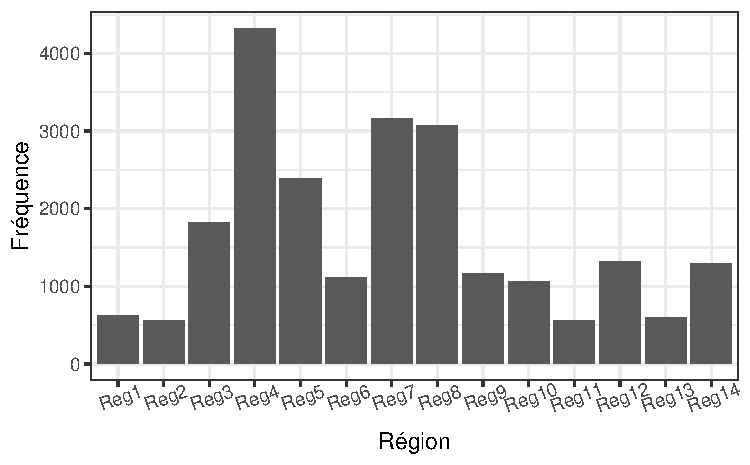
\includegraphics{01-Rapport_files/figure-latex/graph_vehicl_region-1} 

}

\caption{\label{fig:vehiclregion}Distribution des régions habités par les détenteurs de police, représenté par la variable \textbf{vehicl\_region}}\label{fig:graph_vehicl_region}
\end{figure}

\hypertarget{variables-catuxe9gorielles-ordinales}{%
\subsection{Variables catégorielles
ordinales}\label{variables-catuxe9gorielles-ordinales}}

La variable catégorielle ordinale \textbf{prem\_freqperyear} représente
la fréquence par année à laquelle la prime est payable. Les fréquences
possibles sont mensuelles, trimestrielles, semestrielles ou annuelles.

On voit qu'un peu moins de la moitié des clients paie la prime en un
seul versement, environ un quart des clients paient trimestriellement,
et le dernier quart est partagé par la prime payable semestriellement et
mensuellement.

La variable \textbf{vehicl\_powerkw} représente la puissance du moteur
de la voiture conduit exprimé en chevaux moteurs. Initialement, cette
variable contenait 11 niveaux. Cependant, certains niveaux visaient des
valeurs fixes tandis que d'autres étaient définis à l'aide d'intervalle.
Des doublons de niveaux figuraient par défaut dans la liste due à
certains intervalles trop englobants. Afin d'uniformiser la mesure de
cette variable, nous avons regroupé certains niveaux ensemble, soit tous
les niveaux représentant une puissance de 125 à 300 chevaux moteurs.
Cette modification a touché peut de cas était nécessaire pour
l'obtention d'une interprétation adéquate des données. On peut
d'ailleurs observer les proportions de chaque niveau avant et après
modification dans les tables 6 et 7.

\textless\textless\textless\textless\textless\textless\textless{}
HEAD:01-Rapport.Rmd

\begin{table}[ht]
\centering
\caption{Distribution de la puissance du moteur avant et après modification} 
\label{}
\begin{tabular}{lcr}
  \hline
Puissance (kW) & Nombre d'observation & Distribution \\ 
  \hline
25-50 & 4968 & 21.54 \% \\ 
  75 & 10339 & 44.84 \% \\ 
  100 & 5116 & 22.19 \% \\ 
  125-300 & 1720 & 7.46 \% \\ 
  150 & 580 & 2.52 \% \\ 
  175 & 206 & 0.89 \% \\ 
  200 & 32 & 0.14 \% \\ 
  225 & 77 & 0.33 \% \\ 
  250 & 16 & 0.07 \% \\ 
  275 & 4 & 0.02 \% \\ 
   \hline
300 & 2 & 0.01 \% \\ 
  25-50 & 4968 & 21.54 \% \\ 
  75 & 10339 & 44.84 \% \\ 
  100 & 5116 & 22.19 \% \\ 
  125-300 & 2637 & 11.44 \% \\ 
   \hline
\end{tabular}
\end{table}

\newpage

\hypertarget{variables-numuxe9riques-discruxe8tes}{%
\subsection{Variables numériques
discrètes}\label{variables-numuxe9riques-discruxe8tes}}

La variable \textbf{polholder\_age} est une variable numérique discrète
représentant l'âge du propriétaire de la police d'assurance. La
\autoref{fig:polholderAge} représente la distribution d'âges des
assurés.

\begin{figure}

{\centering 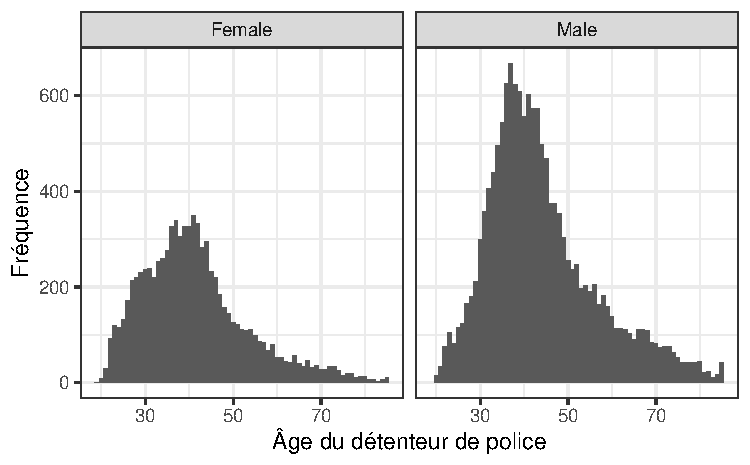
\includegraphics{01-Rapport_files/figure-latex/graph_polholder_age-1} 

}

\caption{\label{fig:polholderAge}Distribution de l'âge des détenteurs de polices dans la base de données, représenté par la variable \textbf{polholder\_age}}\label{fig:graph_polholder_age}
\end{figure}

L'âge des détenteurs de police de cette compagnie d'assurance se situe
entre 19 et 85 ans inclusivement. On constate qu'il y a une forte
proportion d'assurés entre 30 et 45 ans. La distribution est toutefois
similaire que ce soit pour les hommes ou pour les femmes, en gardant en
tête que les hommes sont présent en plus grand nombre. Il pourra être
pertinent d'analyser dans la suite de ce travail pratique si les assurés
de plus de 45 ans sont présents en moins grand nombre dû au fait que les
primes sont trop élevées et compare davantage les primes entre les
divers assureurs sur le marché avant de souscrire à une assurance auprès
de cet assureur directement.

Le nombre d'années sans résignation de la police d'assurance depuis la
première année assurée est représenté par la variable numérique discrète
\textbf{policy\_age}. La \autoref{fig:policyAge} nous permet de
constater que la plupart des assurés renouvellent leur police pour 3
années avant de résigné et une faible partie des assurés renouvelle pour
plus de 3 années de suite. Le maximum est observé à 17 ans.

\begin{figure}

{\centering 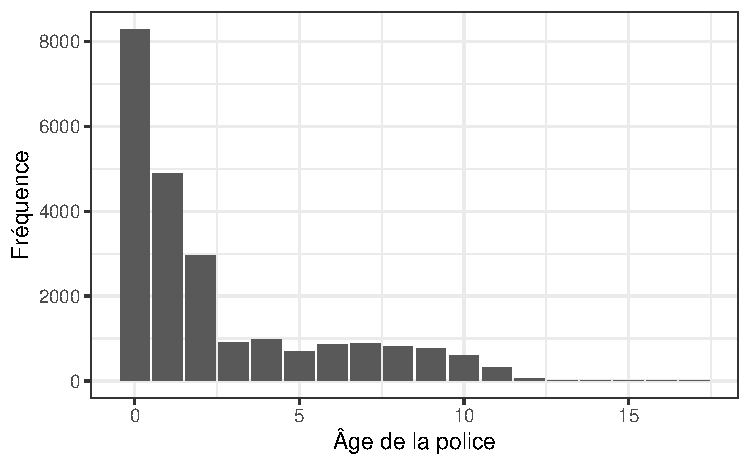
\includegraphics{01-Rapport_files/figure-latex/graph_policy_age-1} 

}

\caption{\label{fig:policyAge}Distribution de l'âge pour laquelle une police est en vigeur, représenter par la variable \textbf{policy\_age}}\label{fig:graph_policy_age}
\end{figure}

En ce qui concerne la variable discrète \textbf{policy\_nbcontract},
elle représente le nombre de contrats que l'assuré possède chez
l'assureur. L'histogramme illustré à la \autoref{fig:policyNbcontract}
fait ressortir le fait qu'il y a une forte concentration d'assuré pour
lesquels le nombre de contrats est inférieur à 5. On peut aussi voir que
certains assurés ont jusqu'à un maximum de 15 contrats.

\begin{figure}

{\centering 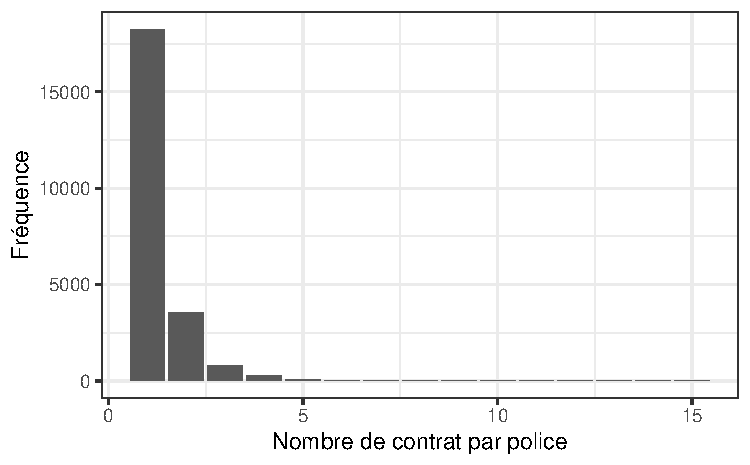
\includegraphics{01-Rapport_files/figure-latex/graph_policy_nbcontract-1} 

}

\caption{\label{fig:policyNbcontract}Distribution du nombre de contrats par police, représenter par la variable \textbf{policy\_nbcontract}}\label{fig:graph_policy_nbcontract}
\end{figure}

Les deux prochaines variables sont en lien avec l'âge du véhicule, il
s'agit de variables numériques discrètes. La variable
\textbf{vehicl\_agepurchase} représente l'âge du véhicule lors de la
transaction pour l'achat du véhicule. La variable \textbf{vehicl\_age}
représente, quant à elle, l'âge actuel du véhicule, soit dans ce cas
l'âge actuel du véhicule au moment où les données ont été prises.

\begin{figure}

{\centering 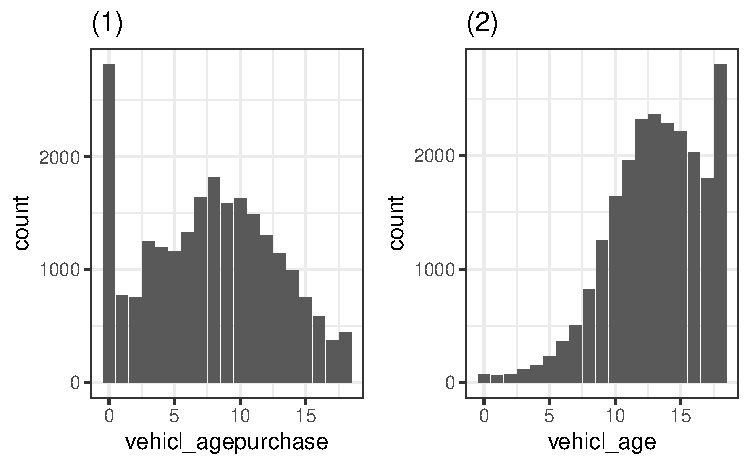
\includegraphics{01-Rapport_files/figure-latex/graph_age-1} 

}

\caption{\label{fig:}Distribution de l'âge des véhicules assurés au moment de l'achat du véhicule comparativement au moment de la prise de données.}\label{fig:graph_age}
\end{figure}

Beaucoup de véhicules ont été achetés lorsqu'il était neuf, soit les
valeurs indiquant 0 an. On remarque également qu'il y a peu de véhicules
neufs lors du moment de la prise de données et que le nombre de
véhicules est croissant en fonction de l'âge actuel jusqu'à 13 ans puis
la tendance inverse est observée pour les âges supérieurs à 13 ans.
Étant donné qu'un véhicule âgé de 18 ans spécifiquement ne devrait
raisonnablement pas être l'âge le plus fréquent, on conclut que cette
valeur comprend 18 ans, mais également tous les âges supérieurs.

\hypertarget{variables-numuxe9riques-continues}{%
\subsection{Variables numériques
continues}\label{variables-numuxe9riques-continues}}

\textless\textless\textless\textless\textless\textless\textless{}
HEAD:01-Rapport.Rmd Il y a plusieurs variables numériques continues
relatives à la prime. La variable \textbf{prem\_final} représente le
montant de la prime proposé pour le renouvellement par l'assureur, la
variable \textbf{prem\_last} représente le montant payé lors du dernier
renouvellement, la variable \textbf{prem\_market} est la prime qui
serait chargée selon le marché et la variable \textbf{prem\_pure}
représente la prime des coûts espérés. Le \autoref{tbl:summaryPrimes1}
montre leur distribution. ======= Il y a plusieurs variables numériques
continues relatives à la prime. La variable \textbf{prem\_final}
représente le montant de la prime proposé pour le renouvellement par
l'assureur, la variable \textbf{prem\_last} représente le montant payé
lors du dernier renouvellement, la variable \textbf{prem\_market} est la
prime qui serait chargée selon le marché et la variable
\textbf{prem\_pure} représente la prime des coûts espérés. Le Tableau 7
montre leur distribution.
\textgreater\textgreater\textgreater\textgreater\textgreater\textgreater\textgreater{}
60809fcbf121cda8bf1ec803d70809dfdf626020:rapport1/01-Rapport.Rmd

Une prime seule peut difficilement expliquer pourquoi un assuré voudrait
résigner sa police d'assurance, car si sa prime est représentative de
son risque réel, il n'aurait pas intérêt à changer d'assureur. Par
contre, si lors de son renouvellement, il voit sa prime grandement
augmenter, il sera davantage sujet à vouloir changer d'assureur pour
réduire ces coûts.

\textless\textless\textless\textless\textless\textless\textless{}
HEAD:01-Rapport.Rmd

\begin{table}[ht]
\centering
\caption{Distribution des quatres types de primes} 
\label{}
\begin{tabular}{lccccc}
  \hline
Prime (\$) & Minimum & Médiane & Moyenne & Maximum & Écart-type \\ 
  \hline
Final & 46.55 & 312.25 & 374.12 & 2948.05 & 212.9 \\ 
  Last & 46.56 & 311 & 380.51 & 3362.07 & 227.94 \\ 
  Market & 50.11 & 316.83 & 373.53 & 2416.84 & 201.92 \\ 
  Pure & 45.55 & 301.45 & 355.88 & 2716.08 & 197.14 \\ 
   \hline
\end{tabular}
\end{table}

Dans les représentations de la \autoref{fig:BoitesMoustache}, on observe
que la distribution des variables \textbf{prem\_last} et
\textbf{prem\_pure} se rapproche de peu en ce qui concerne la moyenne et
la variance des observations. La variable \textbf{prem\_final} diffère
par sa variance plus élevée et la variable \textbf{prem\_market} par sa
moyenne qui est beaucoup plus faible. On remarque également qu'en
général, la variance reliée au détenteur de police de genre féminin est
plus élevée ce qui s'explique par la proportion moins élevée de
détenteurs de police féminins. Pour les moyennes, elles sont semblables
de ce côté, ce qui porte à croire que les primes ne sont pas influencées
par le genre et c'est positif, car ce serait un bais de stéréotype en
cas contraire.

On remarque que les valeurs extrêmes se situent davantage au niveau des
détenteurs de police ayant renouvelé leur contrat, ce qui est
contre-intuitif. Cela porte à croire que ce sont de très mauvais risques
et qu'ils restent assurés auprès de cette compagnie, car une autre
compagnie d'assurance ne pourrait pas leur offrir une meilleure prime.
On peut valider que cette tendance n'est pas seulement reliée à la
méthode de tarification de cette compagnie en comparant la distribution
de \textbf{prem\_last} et \textbf{prem\_market} qui sont très
similaires, ce qui indique que les primes chargées dans cette compagnie
suivent le marché.

On peut également conclure que la prime en valeur absolue ne permet pas
d'expliquer la raison pour laquelle un détenteur de police résignerait
car une prime similaire lui serait chargée chez un autre assureur. Ce
qui poussera réellement un assuré à rechercher un autre assureur, dans
la grande majorité des cas, est son pourcentage d'augmentation au
renouvellement. C'est donc pour cette raison qu'une variable sera créée
pour la suite du travail pratique pour arriver à la modélisation la plus
adéquate possible. Elle sera nommée \textbf{prem\_index} et sera égale à
\textbf{prem\_new} / \textbf{prem\_last} - 1 .

\begin{figure}

{\centering \includegraphics{01-Rapport_files/figure-latex/graph_primes-1} 

}

\caption{\label{fig:BoitesMoustache}Diagrammes en boite à moustache pour les différentes primes selon la variable réponse et le genre du détenteur de la police}\label{fig:graph_primes}
\end{figure}

\newpage

\hypertarget{traitement-des-donnuxe9es-manquantes}{%
\section{Traitement des données
manquantes}\label{traitement-des-donnuxe9es-manquantes}}

La base de données contenait seulement trois variables avec des valeurs
manquantes. La variable indiquant la différence d'âge entre le détenteur
de la police et le conducteur est manquante à 0.05\%, celle indiquant
l'utilité du vehicule est manquante à 15.1\% et la variable indiquant le
type de garage où est entreposé le véhicule est manquante à 6.83\%. La
\autoref{fig:missingPatern} montre le patron de non réponse. On remarque
que la variable \textbf{polholder\_diffdriver} semble avoir un patron de
non réponse monotone avec les deux autres. Par contre, puisqu'il y a
seulement 12 cas, nous n'allons pas tenir compte de ce lien lors de
l'imputation des données. Pour ce qui est des variables
\textbf{policy\_caruse} et \textbf{vehicl\_garage}, on remarque qu'il
sont parfois manquante en même temps, mais seulement pour une minorité
de cas.

\begin{figure}

{\centering 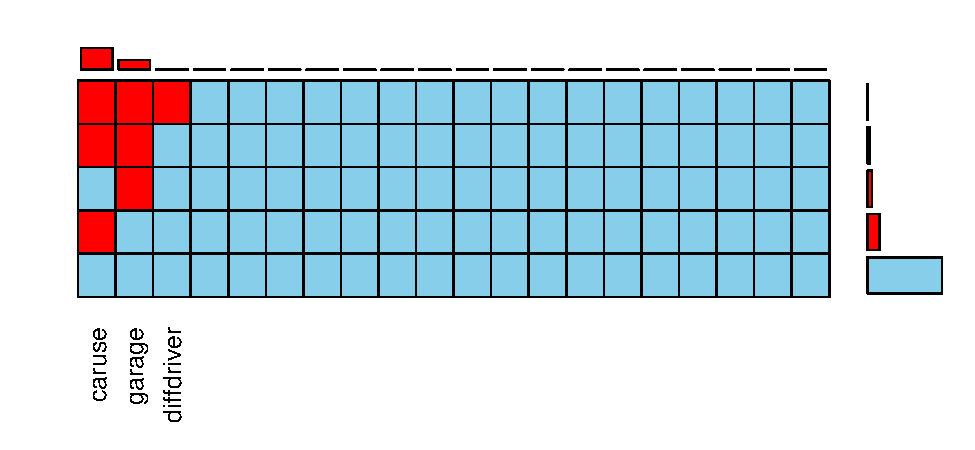
\includegraphics{01-Rapport_files/figure-latex/MissingPattern-1} 

}

\caption{\label{fig:missingPatern}Patron de non réponse}\label{fig:MissingPattern}
\end{figure}

Premièrement, dans le but déterminer si les données manquantes sont
MCAR, le test d'hypothèse suivant a été effectué \begin{align*}
  H_0:&\: \text{Le données sont MCAR} \\
  H_1:&\: \text{Le données ne sont pas MCAR}
\end{align*} Pour conclure que les données sont MCAR, il est nécessaire
d'accepter \(H_0\) pour toutes les variables. Par contre, un seul refus
de cette hypothèse nous permettra de conclure l'hypothèse alternative,
c'est-à-dire que les données ne sont pas MCAR. Pour effectuer le test
avec une variable catégorielle, il sera nécessaire d'utiliser la
statistique de khi carré alors que pour une variable numérique, la
statistique la student sera utilisée.

En ce qui concerne les variables \textbf{vehicl\_garage} et
\textbf{policy\_caruse}, plusieurs statistiques observées permettent de
rejeter l'hypothèse nulle à un niveau significatif de \(0.001%
\). Par contre, dans le cas de \textbf{polholder\_diffdriver}, seulement
la variable \textbf{polholder\_job} permet de rejeter \(H_0\),
c'est-à-dire que les données manquantes ne sont pas complètement
aléatoires.

Il est à noter qu'il n'est pas possible de vérifier avec certitude si
les données sont MAR ou NMAR. Cela est dû au fait que puisque les
données proviennent d'un compagnie inconnue, nous n'avons pas
d'information sur la méthode de récolte des données et il nous est
impossible de trouver des patrons qui pourraient provoquer des données
de type NMAR. En conséquence, nous considérerons que nos données sont
MAR. De ce sens, en effectuant des tests khi-carré pour la variable
\textbf{polholder\_diffdriver}, il a été remarqué que l'information sur
la différence entre le détenteur de police et le conducteur nous indique
que les variables sont toujours manquantes dans le cas ou le travail du
détenteur de la police est dans le domaine de la médecine. Ceci renforce
l'idée que le patron de non-réponse pour cette variable dépend des
variables observées dans le jeu de données, soit que les données sont
NMAR mais nous ne pouvons rien conclure de ce côté.

Pour l'imputation des données, la méthode d'imputation multiple a été
choisie et donc utilisée. Pour des restrictions de temps de calcul, cinq
itérations de régression stochastique ont été faites. Pour la variable
\textbf{policy\_caruse}, une régression logistique a été effectuée
puisque la variable catégorielle comporte deux niveaux. Pour les
variables \textbf{vehicl\_garage} et \textbf{polholder\_diffdriver}, qui
sont des variables catégorielles non ordonnées, une régression
polynomiale a été utilisée.

\newpage

\hypertarget{analyse-en-composantes-principales}{%
\section{Analyse en composantes
principales}\label{analyse-en-composantes-principales}}

Étant donné que notre jeu de données contient
\texttt{R\ nrow(Donnees\_tempo)} observations, il peut être utile de
visualiser les données à l'aide de l'analyse en composantes principales,
appelé ACP. En effet, ce type d'analyse permet de mieux visualiser un
jeu de données lorsque celui-ci est de grande dimension. Il sera ainsi
possible de voir quelles variables explicatives sont plus intéressantes
par leur impact sur la variance des composantes principales. Il est à
noter qu'en général, on garde assez de composantes pour représenter
entre 80 et 90 \% de la variance totale.

Pour que cette méthode de visualisation puisse être utilisée, il sera
nécessaire de prendre seulement les variables explicatives numériques de
ce jeu de donnée. Les variables catégorielles ne seront pas analysées
dans cette section, car même en les transformant en variables
numériques, elles ne seront pas représentatives des valeurs leur qui
leur aurait été attribuée en faisant la modification de type.

On doit ensuite choisir le nombre de composantes principales. Cette
étape peut être complétée en ayant déjà un pourcentage de variance
expliquée en tête et en choisissant le nombre de composantes à partir
des valeurs propres ou en analysant directement le diagramme d'éboulis.
Dans ce cas, la méthode du coude ne sera pas utilisée, on privilégie
davantage le choix selon le premier plateau observé. Le nombre de
composantes choisi seront celles ne faisant pas partie du premier
plateau observé.

\begin{figure}

{\centering 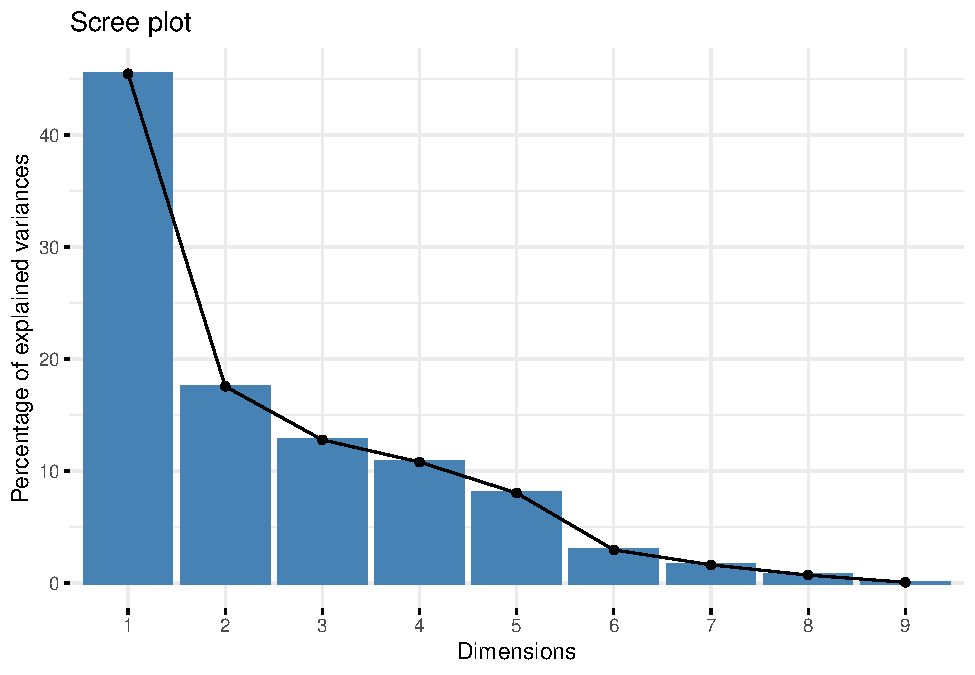
\includegraphics{01-Rapport_files/figure-latex/unnamed-chunk-3-1} 

}

\caption{Diagramme d'éboulis représentant le pourcentage expliquer de la variance pour chaque dimention.}\label{fig:unnamed-chunk-3}
\end{figure}

Selon le diagramme d'éboulis, il sera nécessaire de conserver 2
composantes principales et on observe, à l'aide des valeurs propres de
la matrice de corrélation, que 2 composantes principales permettent
d'expliquer 63\% de la variance totale.

À l'aide du graphique ACP des variables, on peut voir la gravité des
contributions pour chacune des variables sur chaque composante
principale retenue. Ainsi, on peut observer que pour la première
composante principale, un score élevé indique un contrat ayant une prime
élevée, que ce soit la prime du marché, la prime pure, la prime finale
ou la prime chargée lors du dernier renouvellement. Par contre, un
assuré âgé qui renouvelle depuis plusieurs années aura un score plus
faible qu'un assuré en bas âge ayant une police d'assurance récente. Un
score élevé représente donc un assuré en bas âge ayant une police
récente et une prime élevé tandis qu'un score faible représente une
personne plus âgée avec une faible prime d'assurance.

La deuxième composante principale représente, quant à elle, l'âge du
véhicule assuré. Un score élevé est associé à des véhicules de moindres
valeurs, mais risquant davantage un bris de vieillesse. Plus les polices
d'assurance sont récentes et plus le score en sera augmenté. Ainsi, les
polices d'assurance récentes ayant des véhicules de l'année
représenteront les scores les plus faibles pour cette composante.

En illustrant les contributions des variables pour les deux premières
composantes principales, il est plus facile de visualiser les
conclusions mentionnées précédemment.

\begin{figure}

{\centering 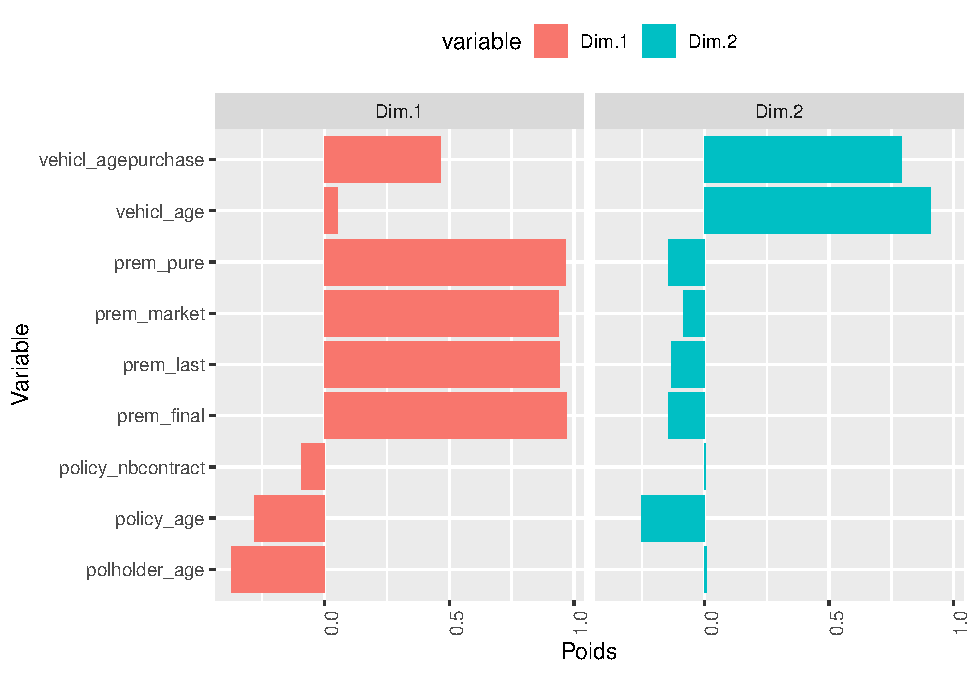
\includegraphics{01-Rapport_files/figure-latex/unnamed-chunk-5-1} 

}

\caption{Représentation de la contribution de chaques variables numériques dans les deux premières dimentions résultant de l'analyse en composante principal.}\label{fig:unnamed-chunk-5}
\end{figure}

\newpage

\hypertarget{partitionnement-en-k-moyennes}{%
\section{Partitionnement en k
moyennes}\label{partitionnement-en-k-moyennes}}

Le partitionnement en k moyennes est utilisé pour classifier les
observations en k groupes distincts. La valeur de k est une valeur qu'on
transmet pour indiquer le nombre de partitions désirées. Chaque
observation sera ensuite assignée à un seul groupe. L'algorithme utilisé
pour ce type de partitionnement a pour objectif de minimiser la variance
intragroupe.

Le choix du nombre de groupe peut être choisi à l'aide de la méthode du
coude. Ainsi en ce référent au graphique suivant, on devrait faire le
partitionnement sur 2 groupes distincts. On s'arrête la valeur de \(k\)
qui ce situe dans le ``pli de coude'', soit juste avant le dernier
plateau du diagramme d'éboulis. Il est à noter que le nombre
d'observations a été réduit pour pouvoir faire le diagramme d'éboulis.
Notre jeu de données étant trop volumineux, ce qui engendrait des
erreurs d'exécution. L'échantillon utilisé a été extrait aléatoirement
et sans remise pour avoir une représentation adéquate et la moins
biaisée possible.

\begin{figure}

{\centering 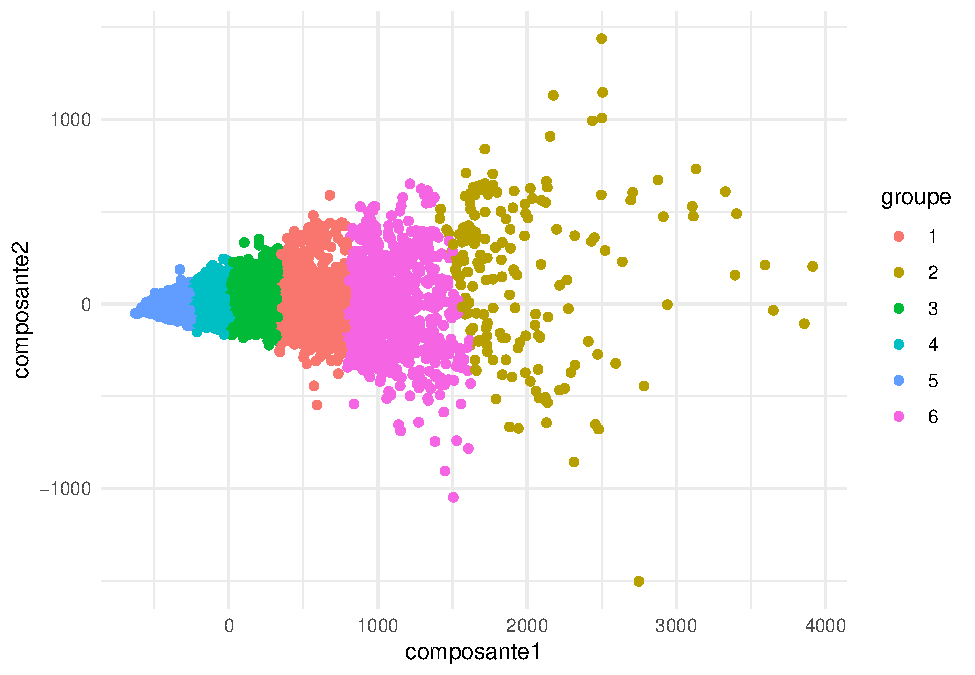
\includegraphics{01-Rapport_files/figure-latex/unnamed-chunk-6-1} 

}

\caption{Diagramme d'éboulis représentant l'erreur intra-groupes pour différent nombre de groupes.}\label{fig:unnamed-chunk-6}
\end{figure}

En ayant en tête le nombre de groupe nécessaire pour la classification,
on effectue le partitionnement et on obtient le graphique présenté à la
\autoref{fig:kmeans}.

\begin{figure}

{\centering 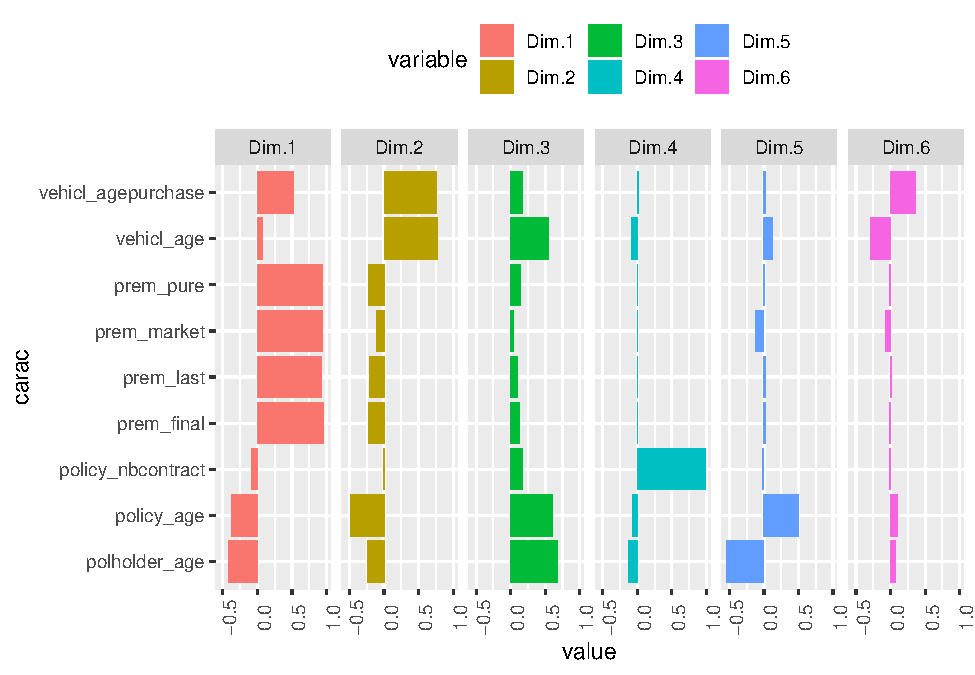
\includegraphics{01-Rapport_files/figure-latex/unnamed-chunk-7-1} 

}

\caption{\label{fig:kmeans}Représentation des deux groupes formés par l'algorithme des $k$-moyenne dans le système d'axe des deux première dimention de l'analyse en composante principal.}\label{fig:unnamed-chunk-7}
\end{figure}

De ce graphique, on peut conclure que le partitionnement s'est fait sur
la première composante principale. Les assurés représentant moins de
risque se retrouve dans le groupe 2 tandis que les assurés plus risqués
se retrouvent dans le groupe 1. Ainsi, le montant des primes typiques
serait d'environ 300\$ ou moins pour le deuxième groupe et de plus de
300\$

\hypertarget{head01-rapport.rmd}{%
\section{\textless\textless\textless\textless\textless\textless\textless{}
HEAD:01-Rapport.Rmd}\label{head01-rapport.rmd}}

\begin{quote}
\begin{quote}
\begin{quote}
\begin{quote}
\begin{quote}
\begin{quote}
\begin{quote}
60809fcbf121cda8bf1ec803d70809dfdf626020:rapport1/01-Rapport.Rmd
\newpage \# Conclusion
\end{quote}
\end{quote}
\end{quote}
\end{quote}
\end{quote}
\end{quote}
\end{quote}

Comme mentionné précédemment, le jeu de données analysé dans ce travail
pratique provient du paquetage ``CASdatasets''. Nous avons choisi ce jeu
de données dans le but de modéliser le statut de renouvellement de
polices d'assurance pour une compagnie et une année d'observation
inconnue. Les variables explicatives touchent les caractéristiques liées
aux primes payées, à l'assuré visé par la police d'assurance et au
véhicule assuré.

Le jeu de donnée de départ a nécessité un prétraitement. Dans cette
étape, nous avons changer le type de la variable réponse ``lapse'' pour
améliorer la visualisation pour la suite. Elle était à prime à bord de
type binaire et nous avons changé le type pour une variable de type
catégorielle nominale prenant les valeurs possibles ``renouvellement''
et ``resignation''. Nous avons également dû changer les valeurs de
certaines variables de ``unknown'' à ``NA'' pour l'uniformité. Les
doublons ont été retirés. La variable \textbf{prem\_freqperyear} a été
réordonnée pour suivre l'ordre logique et améliorer la visualisation. Un
regroupement a, en dernier lieu, été nécessaire, comme expliqué dans
l'analyse exploratoire, dans le but d'uniformiser les différents niveaux
de la variable \textbf{vehicl\_powerkw}. Pour ce qui est de l'analyse
exploratoire des données, cette étape nous a permis de bien visualiser
les distributions et les informations comprises dans chacune des
variables. Nous avons ainsi pu vérifier si des données aberrantes nous
avaient échappées lors des premières modifications apportées. Notre jeu
de données est bien construit et nous permettra d'obtenir un modèle
intéressant. En effet, puisque la variable réponse \textbf{lapse} est
une variable catégorielle pour laquelle deux valeurs sont possibles,
soit renouvellement ou résignation, il sera intéressant pour la suite de
modéliser la probabilité qu'un assuré renouvelle ou résigne pour la
prochaine année. Un modèle linéaire avec régression logistique nous sera
grandement utile pour cette étape. La prédiction de la régression
correspondra, dans ce cas, à la probabilité désirée.

\newpage

\hypertarget{bibliographie}{%
\section{Bibliographie}\label{bibliographie}}

\hypertarget{refs}{}
\begin{cslreferences}
\leavevmode\hypertarget{ref-AnalyseComposantesPrincipales}{}%
Côté, Marie-Pier. 2020a. \emph{ACT-3114 - Analyse En Composantes
Principales}. Recueil inédit; Université Laval.

\leavevmode\hypertarget{ref-ClassificationNonSupervisuxe9e}{}%
---------. 2020b. \emph{ACT-3114 - Classification Non-Supervisée}.
Recueil inédit; Université Laval.

\leavevmode\hypertarget{ref-TraitementDonnesManquantes}{}%
---------. 2020c. \emph{ACT-3114 - Traitement Des Données Manquantes}.
Recueil inédit; Université Laval.

\leavevmode\hypertarget{ref-VisualisationPretraitement}{}%
---------. 2020d. \emph{ACT-3114 - Visualisation et Prétraitement}.
Recueil inédit; Université Laval.

\leavevmode\hypertarget{ref-CASdatasets}{}%
Dutang, Christophe, and Arthur Charpentier. 2019. \emph{CASdatasets:
Insurance Datasets}.
\end{cslreferences}

\newpage

\hypertarget{annexe}{%
\section{Annexe}\label{annexe}}

Description du jeu de données soumis sur le forum :

Notre jeu de données représente le statut de renouvellement pour 23 060
polices d'assurance basées sur un an d'observation. Les données
recueillies proviennent d'une compagnie d'assurance inconnue dont
l'année d'observation est également inconnue.

\end{document}
